% Set up the document
\documentclass{article}

% Page size
\usepackage[
    letterpaper,]{geometry}

% Lines between paragraphs
\setlength{\parskip}{\baselineskip}
\setlength{\parindent}{0pt}

% Math
\usepackage{mathtools}
\usepackage{amssymb}
\usepackage{commath}

% Math notation macros
\def\*#1{\mathbf{#1}}
\newcommand{\dadvd}[2]{\dfrac{\text{D} #1}{\text{D} #2}} % advective derivative

\newcommand{\fS}{\mathcal{S}} % fancy S

\newcommand{\nhat}{\mathbf{\hat{n}}}
\newcommand{\rhat}{\mathbf{\hat{r}}}
\newcommand{\thetahat}{\boldsymbol{\hat{\theta}}}
\newcommand{\xhat}{\mathbf{\hat{x}}}
\newcommand{\yhat}{\mathbf{\hat{y}}}
\newcommand{\zhat}{\mathbf{\hat{z}}}
\newcommand{\omegavec}{\boldsymbol{\omega}}

% Links
\usepackage{hyperref}

% Page numbers at top right
\usepackage{fancyhdr}
\pagestyle{fancy}
\fancyhf{}
\fancyhead[R]{\thepage}
\renewcommand\headrulewidth{0pt}

% Graphics
\usepackage{float}
\usepackage{graphicx}
\graphicspath{ {./img/} }

\begin{document}

\textbf{MATH 462 Assignment 5} \\
\textbf{Matt Wiens \#301294492} \\
\textbf{2020-02-12}

\textbf{A) A Patch of Vorticity.}
Consider an incompressible, but rotational, 2D fluid whose initial
condition is characterized by a circular patch of vorticity
%
\begin{equation*}
    \omega(\*x, 0) =
        \begin{dcases}
            \frac{1}{\pi a^2},& 0 \leq r < a \\
            0,& a < r < \infty
        \end{dcases}
        ,
\end{equation*}
%
where $\omega$ is the $\zhat$-component of vorticity $\omegavec$ and $r
= |\*x|$.

\textbf{i)} Solve for the initial streamfunction $\psi(\*x, 0)$, and
hence determine the initial flow velocity. Your task is simplified in
this geometry since the Poisson PDE for the streamfunction $\psi(\*x,
0)$ is really just an ODE in polar coordinates. Invoke the boundary
values that the flow is bounded at the origin, and decays to zero as $r
\to \infty$. It is also necessary to impose continuity on the
streamfunction and its associated flow at $r = a$. Choose the constant
part of the streamfunction to be zero at $r \to \infty$. Describe the
resulting flow pattern.

\textbf{ii)} Using the vorticity equation, deduce the time evolution of
this flow for $t > 0$. This result, in turn, makes it easy to determine
the pressure field. Invoke the conditions that the pressure approaches a
constant value $p^\infty$ as $r \to \infty$ and is continuous at $r =
a$. Explain why the pressure field is consistent with the flow pattern.

\textbf{iii)} Make a subplot or two showing the important flow
quantities (what should these be?) as a function of $r$.

\textbf{iv)} Finally, show that there is a limiting streamfunction as the patch
parameter $a \to 0$,
%
\begin{equation*}
    \psi_0(\*x, t) = \lim_{a \to 0} \psi(\*x, t)
    .
\end{equation*}
%
Acheson refers to this limit as the line vortex of 3D flow.

\textbf{v)} (This part is optional.) Evaluate two types of circulation
integrals. The first are circular loops centered at the origin with $r =
R$. The second are circular loops that do not enclose (or include) the
origin. One of these evaluations is a calculation; the other is a
mathematical argument.

\newpage

\textit{For this assignment I have collaborated with Paul Balogea.}

\textbf{Solution}

\textbf{i)} First note, at $t = 0$ we have
%
\begin{align*}
    &\omega \zhat = \nabla \times \*u = \nabla \times \del{\dpd{\psi}{y}, - \dpd{\psi}{x}} \\
    &\implies \nabla^2 \psi = - \omega
    .
\end{align*}
%
Since the initial setup of our fluid is radially symmetric we should
assume that the streamfunction $\psi$ does not depend on $\theta$.
Therefore, in polar coordinates our above equation (again, at $t = 0$),
becomes
%
\begin{equation*}
    \psi^{\prime \prime} + \frac{1}{r} \psi^\prime = - \omega
    .
\end{equation*}
%
The solution to this equation is
%
\begin{equation*}
    \psi(r, 0) =
    \begin{cases}
        - \frac{r^2}{4 \pi a^2} + c_1 \log r + c_2, &0 \leq r < a \\
        c_3 \log r + c_4, &a < r < \infty
    \end{cases}
    .
\end{equation*}
%
and hence our initial flow is given by
%
\begin{align*}
    U(x, y, 0) &=
    \begin{cases}
        - \frac{y}{2 \pi a^2} + c_1 \frac{y}{r^2}, &0 \leq r < a \\
        c_3 \frac{y}{r^2}, &a < r < \infty
    \end{cases}
    \\
    \vspace{10mm}
    V(x, y, 0) &=
    \begin{cases}
        \frac{x}{2 \pi a^2} - c_1 \frac{x}{r^2}, &0 \leq r < a \\
        - c_3 \frac{x}{r^2}, &a < r < \infty
    \end{cases}
\end{align*}
%
We will take $c_4 = 0$ as per the instructions. Since the solution must
be bounded at the origin, we must have $c_1 = 0$. To ensure continuity
of the flow/streamfunction we also need $c_3 = - \frac{1}{2 \pi}$. We can
then determine $c_2$ as $c_2 = \frac{-\log a}{2 \pi} + \frac{1}{4 \pi}$
Hence our flow simplifies to
%
\begin{align*}
    U(x, y, 0) &=
    \begin{cases}
        - \frac{y}{2 \pi a^2}, &0 \leq r < a \\
        - \frac{y}{2 \pi r^2}, &a < r < \infty
    \end{cases}
    ,
    \\
    \vspace{10mm}
    V(x, y, 0) &=
    \begin{cases}
        \frac{x}{2 \pi a^2}, &0 \leq r < a \\
        \frac{x}{2 \pi r^2}, &a < r < \infty
    \end{cases}
    .
\end{align*}
%
In the Figure~\ref{fig:ai} below the flow is shown. We can see that the
flow is circular, with the magnitude of the flow increasing from the
origin to $r = a$, and then decaying again past $r = a$ (although more
slowly).
%
\begin{figure}[!ht]
    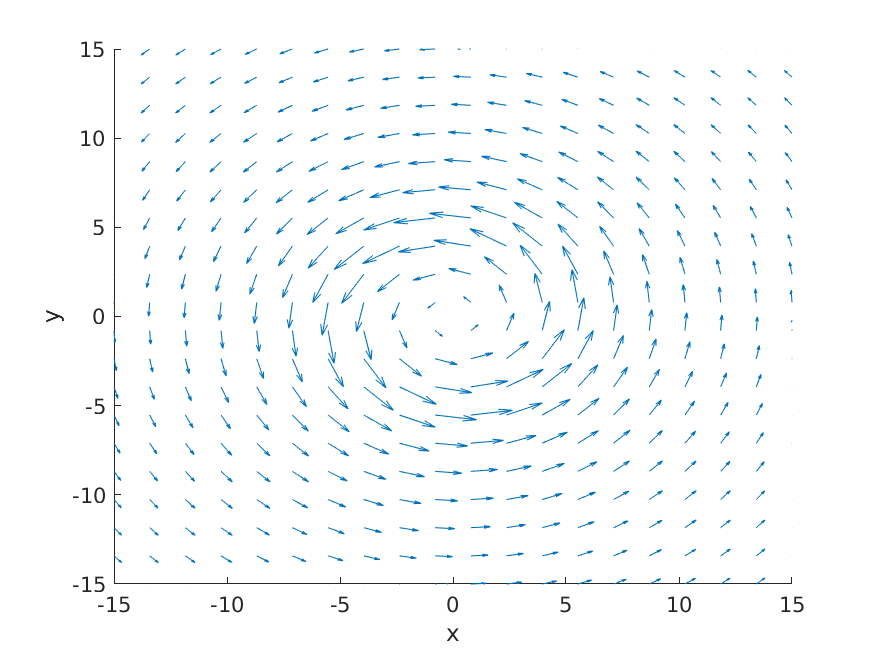
\includegraphics[width=30em]{as05fig1}
    \centering
    \caption{The resulting flow with $a = 5$}
    \label{fig:ai}
\end{figure}

\textbf{ii)} Using the vorticity equation for a 2D flow we have
%
\begin{equation*}
    \dpd{\omega}{t} + (\*u \cdot \nabla) \omega = 0
    .
\end{equation*}
%
On both regions $0 \leq r < a$ and $a < r < \infty$ we have $\nabla
\omega = 0$ at $t = 0$, since in either case it is just a constant.
Hence we can deduce from the above equation that $\dpd{\omega}{t} = 0$
for all time.

Hence the vorticity $\omegavec$ and thus the streamfunction $\psi$ end
velocity $\*u$ is constant in time. Using the equation
%
\begin{equation*}
    \dpd{\*u}{t} + \omegavec \times \*u = - \nabla \del{\frac{p}{\rho_0} + \frac{1}{2} |\*u|^2}
\end{equation*}
%
we can solve for the pressure $p$. Noting that $\dpd{\*u}{t} = 0$ we can
break down this equation into components:
%
\begin{align*}
    \omega V &= \frac{p_x}{\rho_0} + U U_x + V V_x, \\
    - \omega U &= \frac{p_y}{\rho_0} + U U_y + V V_y
    .
\end{align*}
%
Solving for the pressure $p$, we get that, for constants $c$ and $d$,
%
\begin{equation*}
    p =
    \begin{dcases}
        \frac{\rho_0 r^2}{8 \pi^2 a^4} + c, &0 \leq r < a \\
        - \frac{\rho_0}{8 \pi^2 r^2} + d, &a < r < \infty
    \end{dcases}
\end{equation*}
%
The constant $d$ is $p^\infty$ as was instructed by the question description. The
constant $c$ we can determine through continuity at $r = a$, which gives us
%
\begin{equation*}
    c = - \frac{\rho_0}{4 \pi^2 a^2} + p^\infty
    .
\end{equation*}
%
This pressure (as can be seen in Figure~\ref{fig:aiii} below), is
consistent with the fluid flow, since, as was described in lectures, the
pressure differential causes the flow to curve towards the lower
pressure region. Because this pressure differential is radially
symmetric, the flow curvature is radially symmetric everywhere, which is
what we observe.

\textbf{iii)} Figure~\ref{fig:aiii} shows a heat map of the pressure and
fluid flow with $a = \rho_0 = p^\infty = 1$.
%
\begin{figure}
    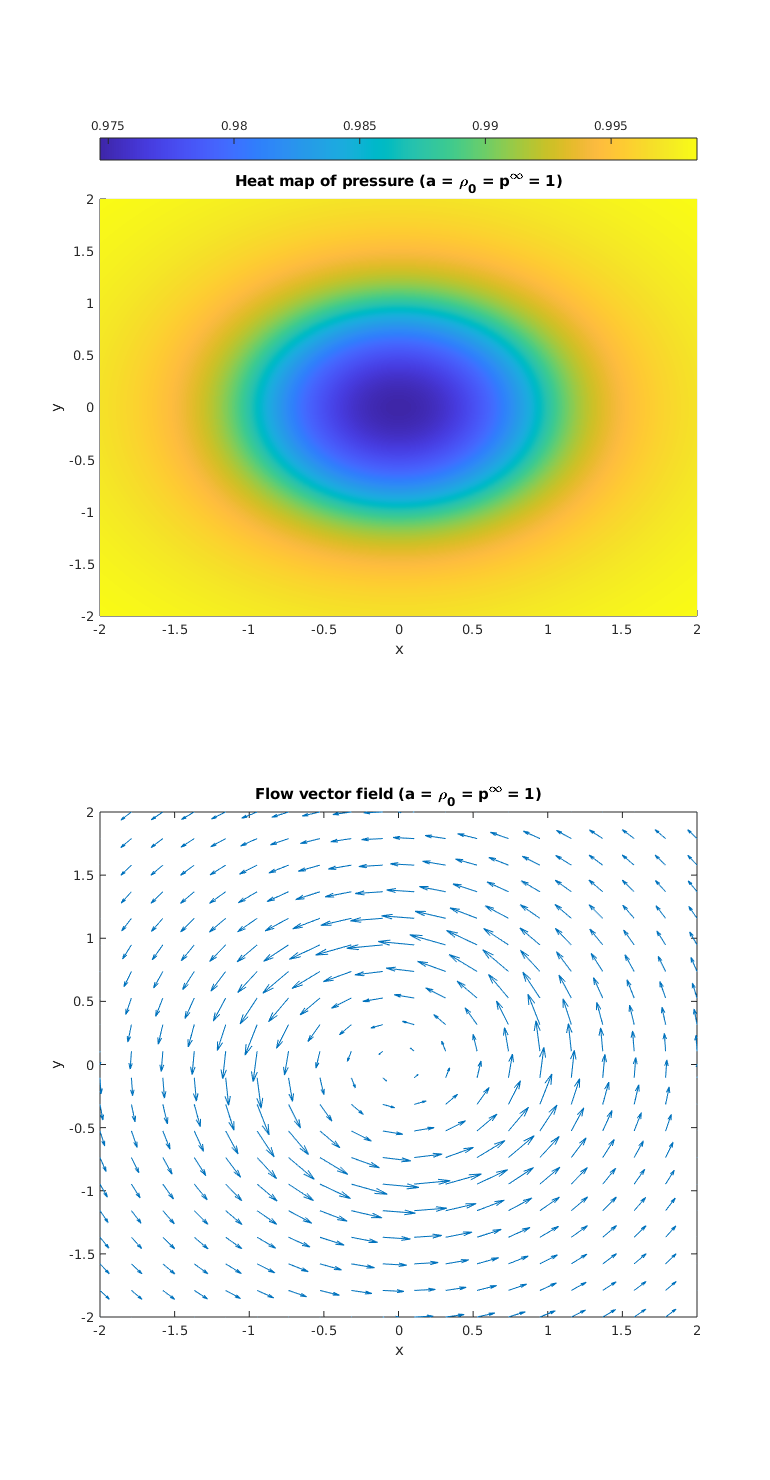
\includegraphics[width=95mm]{as05fig2}
    \centering
    \caption{Subplots of flow quantities}
    \label{fig:aiii}
\end{figure}

\textbf{iv)} Finally, note that for the limiting streamfunction $\phi_0$
we can essentially discard the $0 \leq r < a$ region (since $a \to 0$),
and therefore
%
\begin{equation*}
    \phi_0(\*x, t) = \lim_{a \to 0} \phi(\*x, t) = - \frac{1}{2 \pi} \log |\*x|
\end{equation*}

\newpage

\textbf{B) Circulation as a constant of the Flow.}
The circulation integral was introduced for its connection to the
vorticity via the Stokes theorem,
%
\begin{equation*}
    \Lambda_{\partial \fS}
        = \oint_{\partial \fS (t)} \*u \cdot \dif \*x
        = \iint_{\fS} \del{\nabla \times \*u} \cdot \nhat \dif S
        ,
\end{equation*}
%
where $\partial \fS$ is a simple closed curve within the flow that is a
boundary for the open surface $\fS$. However, when this integral
$\Lambda_{\partial \fS (t)}$ is considered on a curve being advected by
the flow, the idea of circulation is elevated in importance by the
Kelvin circulation theorem. As in the opening of Chapter 5 in Acheson,
the theorem is the conservation principle
%
\begin{equation*}
    \dod{}{t} \Lambda_{\partial \fS (t)} = 0
    .
\end{equation*}
%
The justification is contained in the chapter (partially as Problem
5.2), but you are being asked to derive this result using a mathematical
difference quotient approach, with proper limits being stated. Follow
the outline and the cartoon sketch below.
%
\begin{figure}[!ht]
    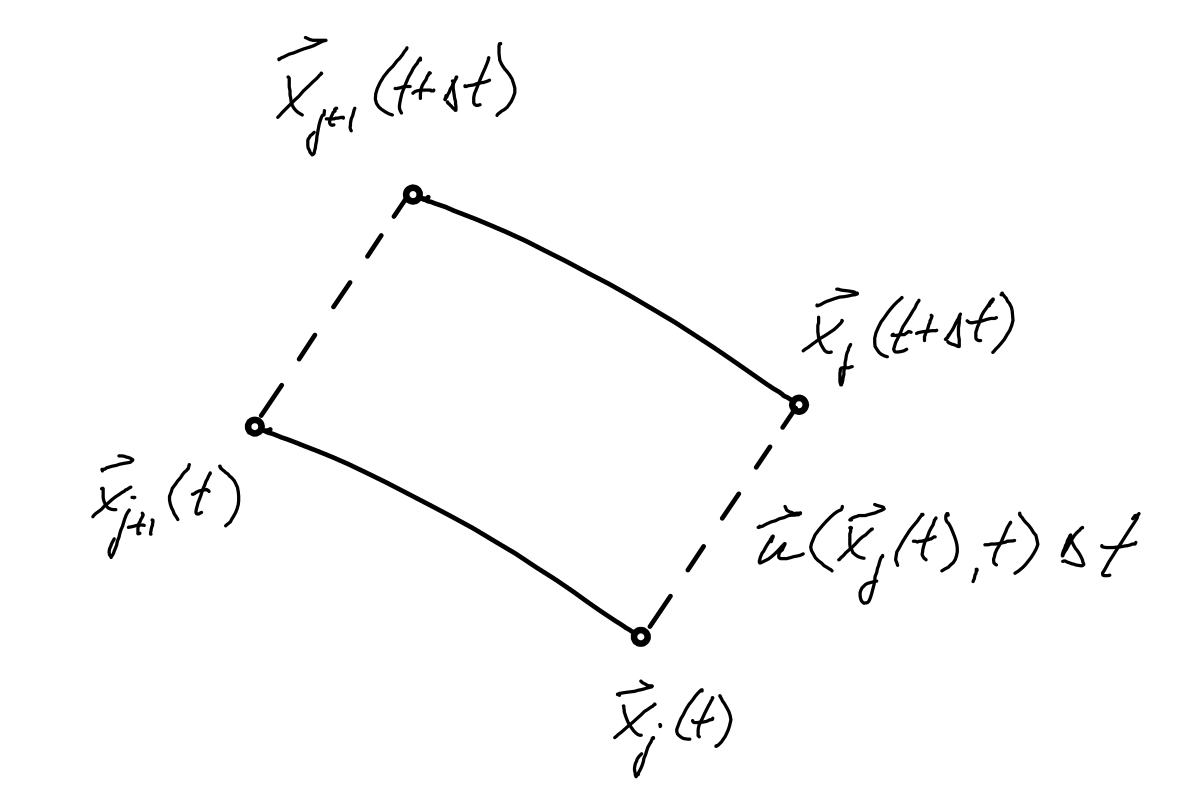
\includegraphics[width=14em]{b-diag}
    \centering
\end{figure}

1) Express the integral
%
\begin{equation*}
    \Lambda_{\partial \fS (t)} = \oint_{\partial \fS} \*u(\*x, t) \cdot \dif \*x
\end{equation*}
%
as a Riemann sum over the intervals $\Delta \*x_j = \*x(t)_{j + 1} -
\*x(t)_j$ where $|\Delta \*x_j| \to 0$ gives the limit to the integral.
But what value should you use for the $\*u$? It really doesn't matter,
but the most robust choice for many will be the trapezoidal rule that
takes the average between the values at $\*x(t)_j$ and $\*x(t)_{j + 1}$.

2) Now write the Riemann sum for the circulation integral at $t + \Delta
t$, and form the difference quotient for the $t$-derivative.

3) The difference quotient expression can be broken up into two sums,
only one of which immediately has the form of a Riemann sum. Evaluating
the limits associated with this Riemann sum results in the derivation as
sketched out in Acheson.

4) But what about the other sum? This is where the midpoint rule works
its magic---it forms a telescoping sum. And since the integral is
over a closed loop, the net contribution is zero!

\newpage

\textbf{Solution}

1. We can express the integral using Riemann sums, separating $\partial
   \fS$ into $n$ line segments, where for notational purposes we set
   $\*x_{n + 1} = \*x_0$.
%
\begin{align*}
    \Lambda_{\partial \fS (t)}
        &= \oint_{\partial \fS} \*u(\*x, t) \cdot \dif \*x \\
        &\approx \sum_{i = 1}^n \*u(x_i, t) \cdot \Delta \*x_i(t) \\
        &\approx \frac{1}{2} \sum_{i = 1}^n \del{\*u(x_i, t) + \*u(x_{i + 1}, t)} \cdot \Delta \*x_{i}(t)
        ,
\end{align*}
%
where in the last step we used the suggested trapezoidal rule for $\*u$.

2. For time $t + \Delta t$, we have the corresponding integral
%
\begin{align*}
    \Lambda_{\partial \fS (t + \Delta t)}
        &\approx \frac{1}{2} \sum_{i = 1}^n \del{\*u(\*x_i, t + \Delta t) + \*u(\*x_{i + 1}, t + \Delta t)} \cdot \Delta \*x_i(t + \Delta t)
        .
\end{align*}
%
To approximate the $t$-derivative, we can use the difference quotient
%
\begin{align*}
    &\frac{\Lambda_{\partial \fS (t + \Delta t)} - \Lambda_{\partial \fS (t)}}{\Delta t} \\
        &\approx \frac{1}{2 \Delta t} \sum_{i = 1}^n
            \del{
                \del{\*u(\*x_i, t + \Delta t) + \*u(\*x_{i + 1}, t + \Delta t)} \cdot \Delta \*x_i(t + \Delta t)
                - \del{\*u(\*x_i, t) + \*u(\*x_{i + 1}, t)} \cdot \Delta \*x_{i}(t)
            } \\
        &= \frac{1}{2 \Delta t} \sum_{i = 1}^n
            \del{
                \*u(\*x_i, t + \Delta t) \cdot \Delta \*x_i(t + \Delta t)
                - \*u(\*x_i, t) \cdot \Delta \*x_i(t)
            } \\
        &\qquad + \frac{1}{2 \Delta t} \sum_{i = 1}^n
            \del{
                \*u(\*x_{i + 1}, t + \Delta t) \cdot \Delta \*x_i(t + \Delta t)
                - \*u(\*x_{i + 1}, t) \cdot \Delta \*x_i(t)
            }
        .
\end{align*}

3. In the previous part we broke up the sum into two parts. The first
   part, by taking the $\Delta \*x \to 0$ we have
%
\begin{equation*}
    \frac{1}{2 \Delta t} \sum_{i = 1}^n
        \del{
            \*u(\*x_i, t + \Delta t) \cdot \Delta \*x_i(t + \Delta t)
            - \*u(\*x_i, t) \cdot \Delta \*x_i(t)
        } \to \dod{}{t} \oint_{\partial \fS} \*u(\*x, t) \cdot \dif \*x
        .
\end{equation*}
%
4. I'm honestly not sure where the magic in this part is. I tried
   working something out for awhile, but couldn't come up with anything.

\end{document}
